\section{Introduction}
\label{sec:intro}
A leaderboard rank does not tell you how a driving policy will behave in a new domain. End-to-end and vision-language-action (VLA) driving policies are compared by benchmark scores, and a deployment decision is, implicitly, a bet that the rank those scores produce will still hold once the policy is driving at the new site, not just on someone else's roads.
On scenes where a pedestrian is near the ego corridor, that bet fails for the six released policies we test: their rank on nuScenes'~\cite{caesar2020nuscenes} open-loop error or on NAVSIM's~\cite{dauner2024navsim} leaderboard score does not carry over to the deployment site (rank correlation $|\rho|\le\NumStdRhoMax$ against near-pedestrian behaviour there, \cref{sec:sample}), a gap that open-loop scores are known to open~\cite{zhao2026bridgesim,li2024egostatus,codevilla2019exploring}. The reason is not noise but mechanism. A score is an outcome measure, and an outcome can be right for the wrong reason: a policy that never approaches a pedestrian because it plans short trajectories scores as well as one that sees the pedestrian and yields, and the two behave very differently the first time the scene changes. Telling them apart means asking why the score came out as it did, usually from little data, because a closed-loop simulator for the target domain or a fleet test is exactly what the decision is meant to save.

Deployment safety cases still rest on target-domain miles~\cite{kusano2025waymo56m}, and post-training on a policy's own deployments~\cite{pi2025pistar06} presumes the same access. For a selection decision, that cost is prohibitive~\cite{kalra2016driving}.

Cross-domain work in domain adaptation~\cite{ganin2015dann} and generalisation~\cite{gulrajani2021lost}
solves the shift through training and does not assess how a policy behaves in the target domain, so
it leaves the selection problem at deployment open.

Closer to our setting, \cite{kachaev2025don} improves a VLA's out-of-distribution generalisation by
aligning its visual representations, but it presumes an already-chosen vision--language model and
offers no procedure for selecting among policies, vision-only ones included. Representation engineering~\cite{zou2023repe} locates and steers concepts in a language model's activations, but it is built around text prompts. Function
vectors~\cite{todd2024functionvectorslargelanguage} show that a task can be read out of, and
transferred through, a language model's hidden states. We know of no counterpart of these instruments for the cross-domain evaluation of driving policies.

\begin{figure*}[!t]
\centering
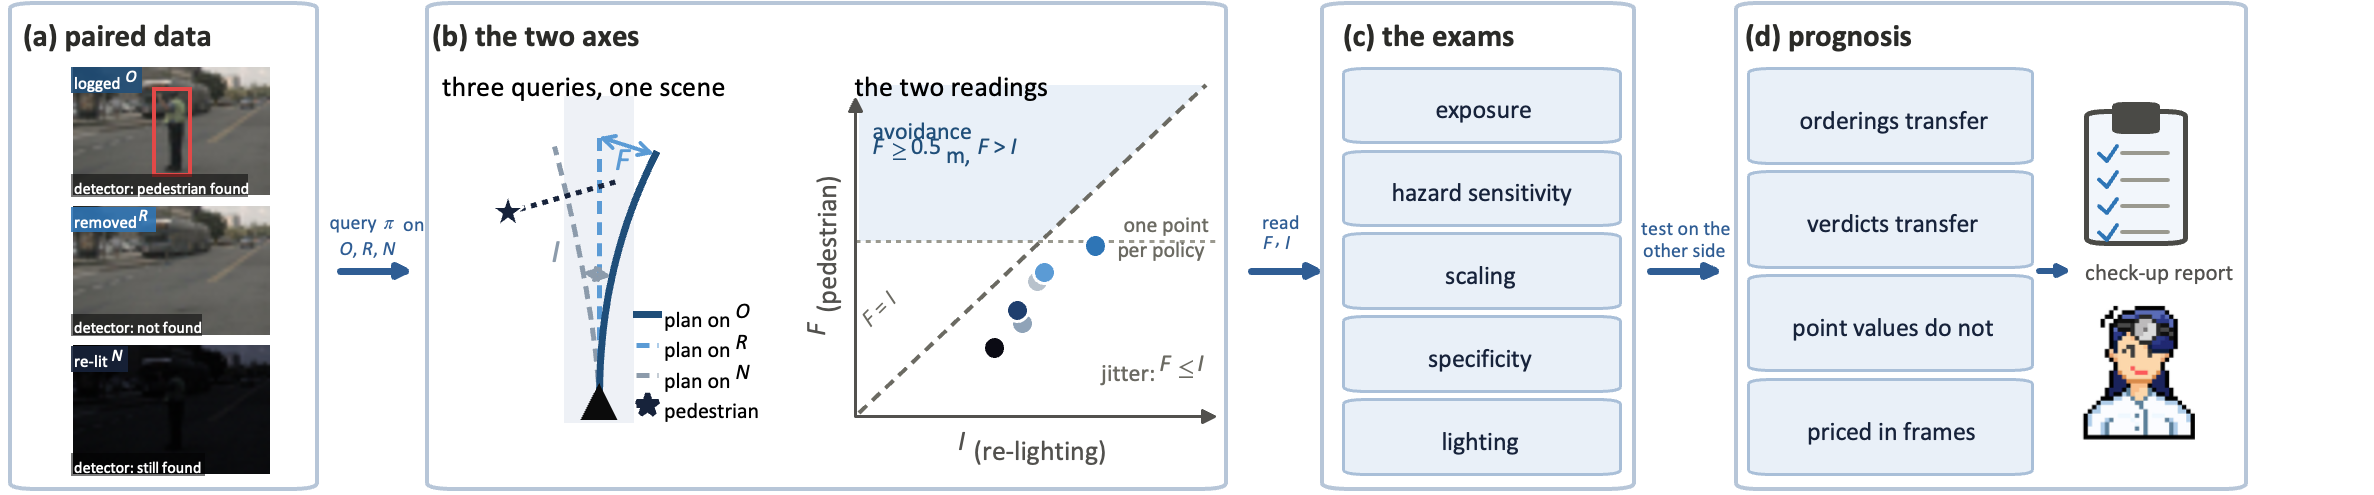
\includegraphics[width=\textwidth]{figures/frame_user.png}

\caption{\textbf{The Check-Up framework.} Pixel-level paired data (a) yield the two causal axes (b) and the five exams built on them (c). Diagnosed on one driving side and tested on the other, they give a priced prognosis, the check-up report (d).}

\label{fig:method}
\end{figure*}
To address this, we propose the \emph{Check-Up}, a counterfactual diagnosis in four stages (\cref{fig:method}). (a)~We construct pixel-level paired data: every logged frame is queried with and
without the target pedestrian and under a night-style photometric perturbation, and an
independent detector verifies every edit. (b)~From each pair we distil two axes of causal
attribution---the \emph{faithfulness} displacement $F$, the plan change caused by the pedestrian
itself, and the \emph{interference} displacement $I$, the change the same policy produces under an
edit that carries no driving-relevant information~\eqref{eq:FI}. (c)~Five exams, each with a control and a reference threshold, are built on these paired plans and axes (\cref{fig:method}c): how far the policy plans
to drive, whether seeing the pedestrian buys safety, whether that benefit scales with the hazard,
whether the plan moves when nothing requires it, and how much the irrelevant edit moves it. (d)~Read on one driving side and tested on the other, the exams yield a prognosis for the target domain: which verdicts and orderings carry over, what each verdict costs in frames, and a per-policy selection report.

The contribution is the Check-Up, a counterfactual diagnosis of end-to-end and VLA driving
policies under domain shift, in three parts.
\begin{enumerate}\itemsep2pt
\item \emph{Pixel-level paired data.} Every logged frame is queried with and without the target
      pedestrian and under a night-style perturbation, each edit verified by an
      independent detector. Six released policies are read on two driving sides.
\item \emph{Two causal axes.} A response is read as the faithfulness displacement $F$ and the
      interference displacement $I$~\eqref{eq:FI}, and counts as avoidance only if it moves and buys distance, and exceeds the interference where a re-lit plan exists. Where the pedestrian lies on the planned path, \NumCfRealPct\%
      of responses qualify, and the lighting edit moves every plan further than the pedestrian does.
\item \emph{A priced prognosis.} Diagnosed on one driving side and tested on the other, the exposure and specificity orderings, the lighting verdict and the collision outcome transfer, while point values and the hazard-sensitivity verdict do not. Each verdict is priced in frames, lighting within \NumNstarCFRhi, exposure within \NumNstarExpHi, and the profiles read as a selection report that says what each policy needs before deployment (\cref{sec:sample}).
\end{enumerate}

